\chapter{一条轨迹的抽样}
\label{app:trace}

本章只读 \texttt{demo\_seed7\_dual.csv}。条件是肉糜、厚度 30 mm、初温 \(8^\circ\mathrm{C}\)、初始含水 0.72、均匀、种子 7、对偶策略、时域 55 min。记录间隔 8 s。它不是中位数，也不代替交叉表。

\section{探针前后}

方差在 192 s 从 0.64 降到 0.224，比值 \(0.224/0.64=0.35\)，与“更接近参照时把方差乘 0.35”一致。蒸汽指令只在 152 s、160 s、168 s 三个记录点为 1。冷点在这 40 s 里从 \(8.01^\circ\mathrm{C}\) 到 \(8.05^\circ\mathrm{C}\)。表面从 \(80.1^\circ\mathrm{C}\) 到 \(88.6^\circ\mathrm{C}\)。短窗口没有推动冷点，这是这一条轨迹上的事实，不是厚度定律。

估计冷点在第一个记录点是 \(-7.92^\circ\mathrm{C}\)。先验 \(\hat r=5\) 时，滞后上限从表面读数减去 \(4\times(5-1)=16\,\mathrm{K}\)。初温附近的表面读数减去 16 K 就是负值。负值表示“还不能把表面当成冷点”，不是传感器测到了零下。

\begin{table}[ht]
\centering
\caption{种子 7、对偶、肉糜 30 mm 的抽样（摄氏度）}
\begin{tabular}{rrrrrrrr}
\toprule
\(t/\mathrm{s}\) & 表面 & 冷点 & 估计 & \(\alpha_m\) & \(\mathrm{Var}\) & 加热 & 模式 \\
\midrule
0 & 11.36 & 8.00 & \(-7.92\) & 0 & 0.640 & 1.00 & 品质 \\
152 & 80.10 & 8.01 & \(-1.45\) & 0 & 0.640 & 1.00 & 探针 \\
168 & 87.12 & 8.02 & \(-0.49\) & 0 & 0.640 & 1.00 & 探针 \\
192 & 88.60 & 8.05 & 0.99 & 0 & 0.224 & 1.00 & 品质 \\
600 & 132.22 & 16.22 & 25.76 & \(\approx 0\) & 0.224 & 1.00 & 品质 \\
1200 & 163.97 & 46.72 & 63.76 & 0.003 & 0.224 & 1.00 & 品质 \\
1496 & 148.76 & 63.31 & 79.57 & 0.131 & 0.224 & 0.56 & 品质 \\
1680 & 128.12 & 73.00 & 85.85 & 0.755 & 0.224 & 0.15 & 保持 \\
1800 & 110.28 & 78.50 & 88.07 & 0.996 & 0.224 & 0.15 & 保持 \\
3298 & 80.84 & 80.85 & 61.05 & 1.000 & 0.224 & 0.15 & 保持 \\
\bottomrule
\end{tabular}
\end{table}

1680 s 这一行是模式从品质切到保持的记录点。估计 \(85.85^\circ\mathrm{C}\)，冷点 \(73.00^\circ\mathrm{C}\)，\(\alpha_m=0.755\)。相对设计线，\(e_{\alpha}=0.755-0.85=-0.095\)。停机判据看的是估计温度越过 \(75\) 加裕量，不是真值进度已经越过 0.85。此后加热请求降到 0.15，真值进度仍继续升到 1。终点进度不能代替停机进度。

1200 s 时估计 \(63.8^\circ\mathrm{C}\) 高于冷点 \(46.7^\circ\mathrm{C}\)。滞后上限没有在整条轨迹上保持估计低于冷点。原因是上限用表面读数减一项只依赖 \(\hat r\) 的常数，表面已经远高于冷点之后，估计仍可以停在冷点之上。这一条轨迹说明：已实现的跟踪器不是冷点的下置信界。交叉表里中等厚度对偶的中位误差接近零、厚件仍然为负，要放在这个观测器的偏差结构上看，不能写成无偏停止。

\section{同一格式重放的内部场}

CSV 只保存表面、冷点最小值和估计。十六条控制体的剖面不在文件里。用附录 \ref{app:discrete} 的离散格式，以同一初值、同一策略和同一噪声重放，表面、冷点和估计与 CSV 的最大差都低于 \(5\times 10^{-6}\,\mathrm{K}\)。差来自写文件时保留五位小数。对齐之后，重放的内部场可以和这条轨迹放在一起读。它仍然是一条轨迹，不是 4860 条的中位剖面。

\begin{figure}[ht]
\centering
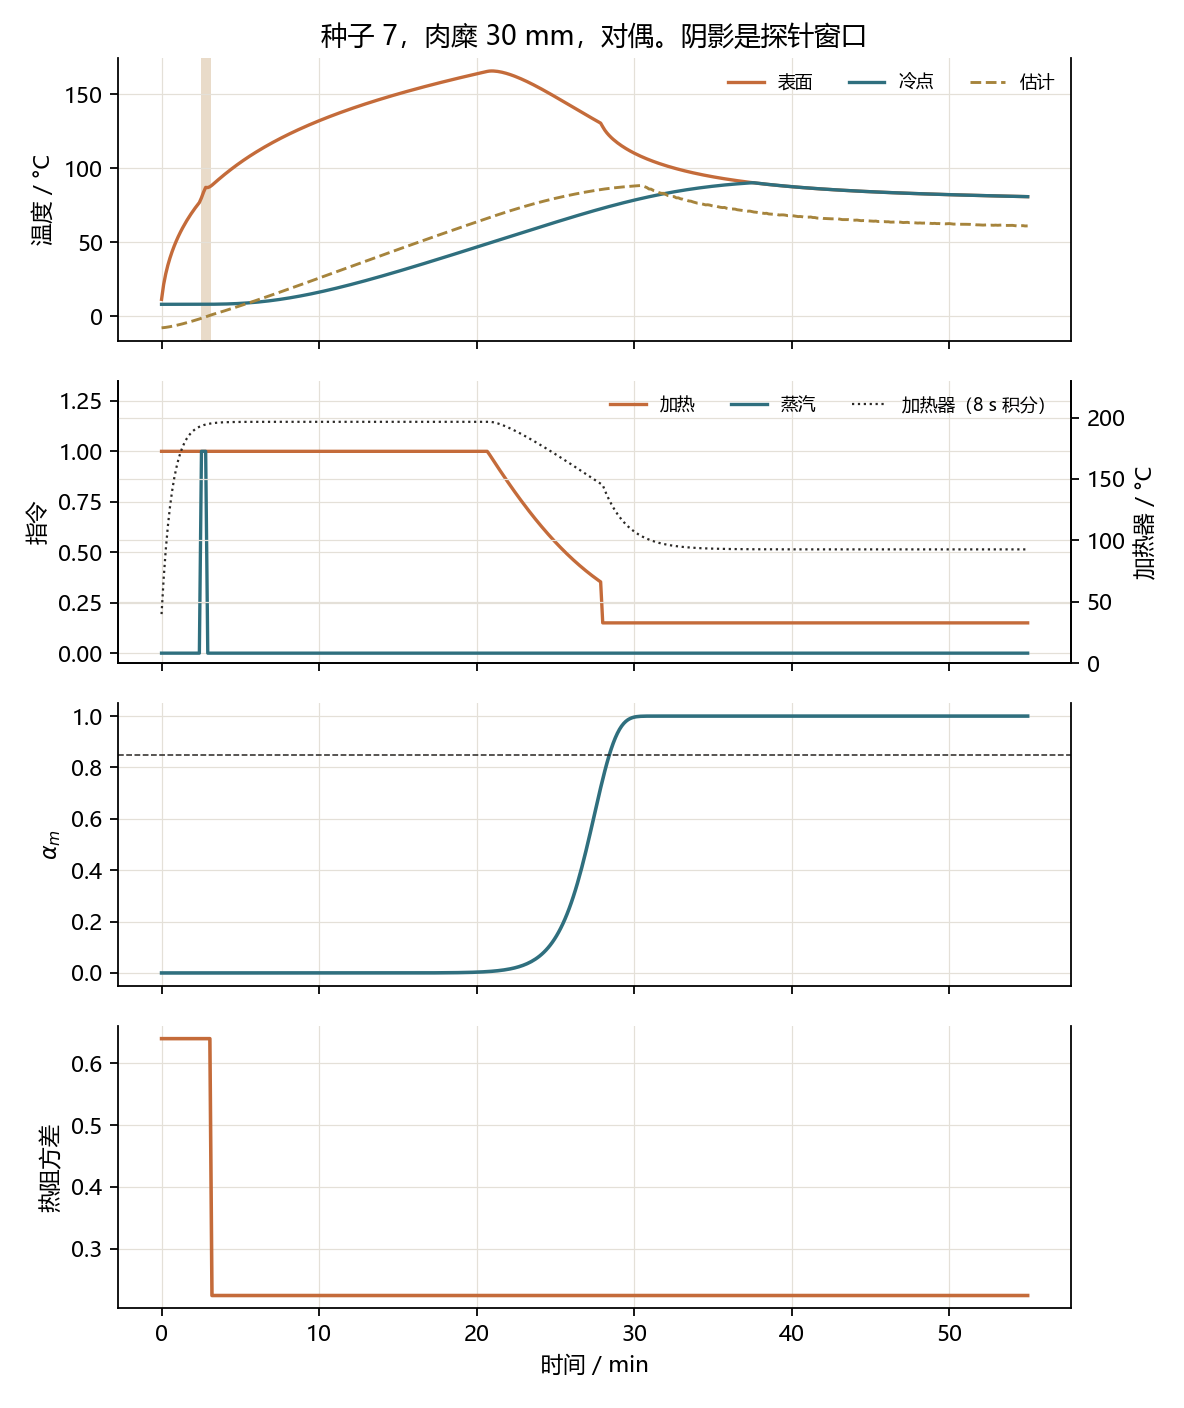
\includegraphics[width=\textwidth]{paper/P_seed7_panels.png}
\caption{种子 7 的四层记录。阴影是 150--190 s。加热器曲线用记录间隔 8 s 积分同一条加热指令，平衡仍是 \(196.5^\circ\mathrm{C}\)，不到 \(230^\circ\mathrm{C}\)。蒸汽脉冲在这张时间轴上只占很窄的一段。}
\end{figure}

\begin{figure}[ht]
\centering
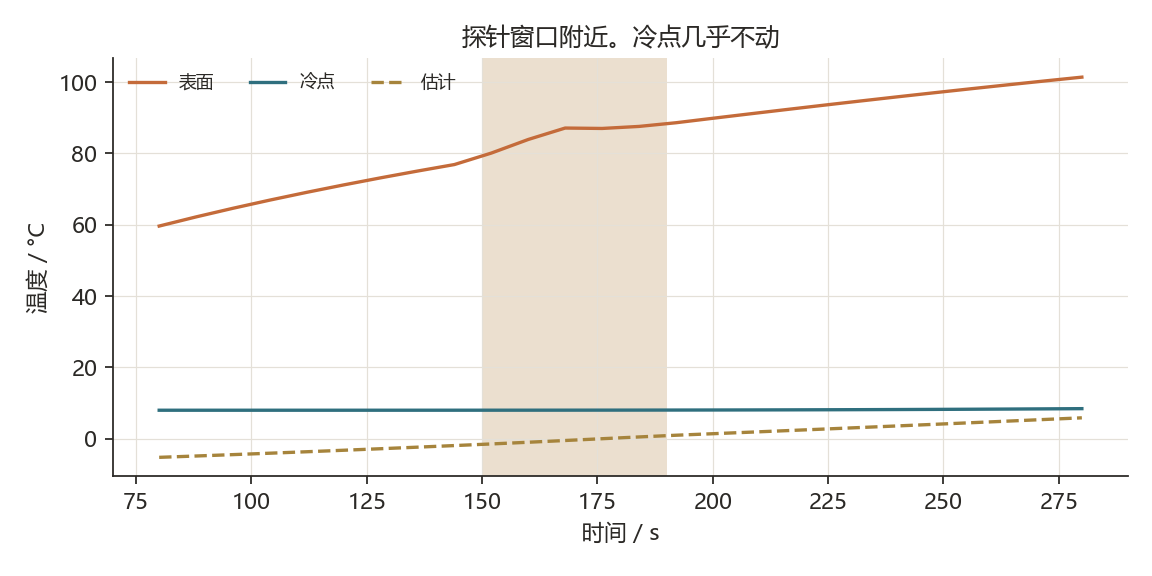
\includegraphics[width=0.92\textwidth]{paper/P_probe.png}
\caption{探针窗口附近。冷点保持在初温附近，表面已经升过 \(80^\circ\mathrm{C}\)。}
\end{figure}

\begin{figure}[ht]
\centering
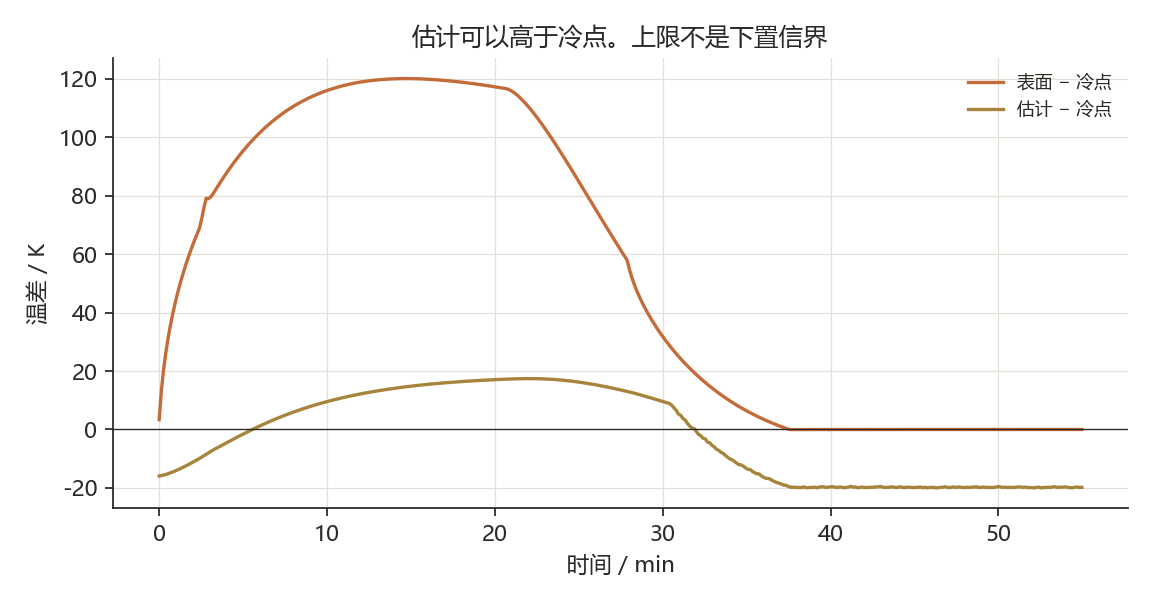
\includegraphics[width=0.92\textwidth]{paper/P_gap.png}
\caption{表面与冷点的温差，以及估计与冷点的温差。后一条曲线在中段为正，估计高于冷点。}
\end{figure}

\begin{figure}[ht]
\centering
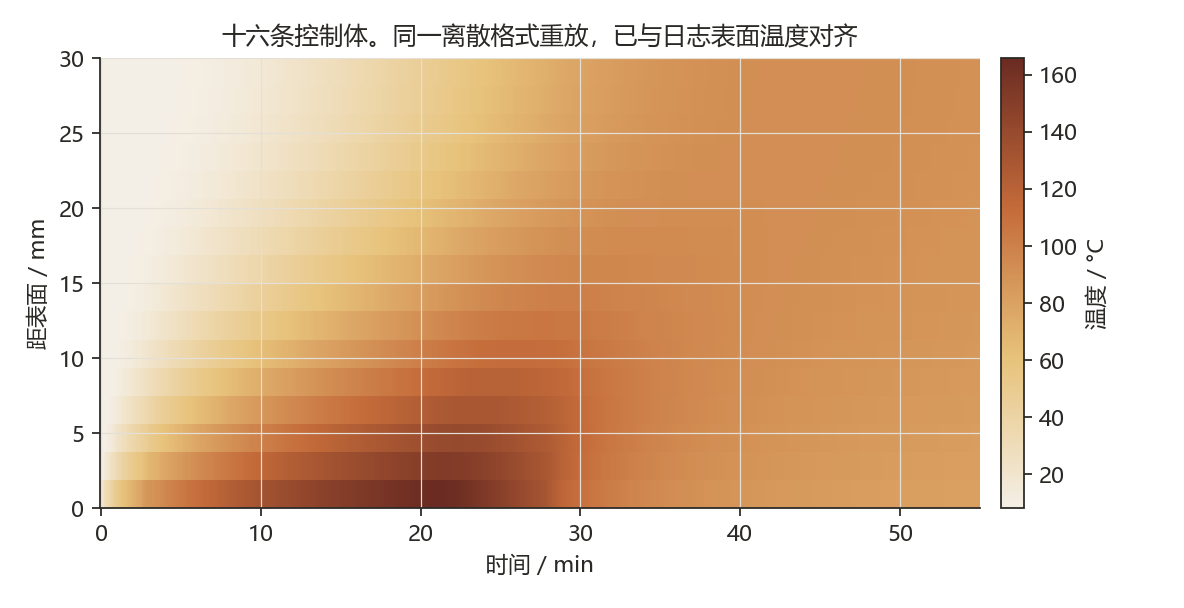
\includegraphics[width=\textwidth]{paper/P_field_xt.png}
\caption{重放得到的温度。纵轴是距表面的距离。高温区先出现在表面，冷点在深处，停机之后全厚度回落。这不是二维烤箱的切片。}
\end{figure}

\begin{figure}[ht]
\centering
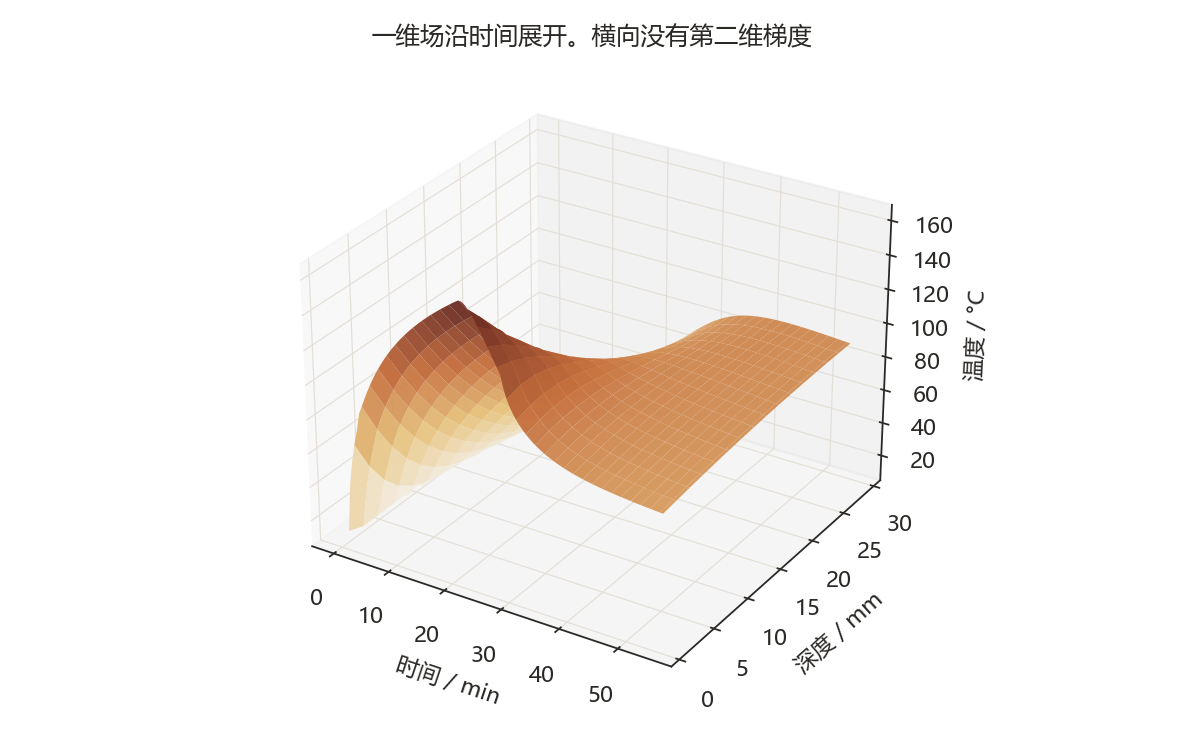
\includegraphics[width=0.88\textwidth]{paper/P_field_3d.png}
\caption{把同一条一维剖面沿时间立起来。深度轴上没有横向梯度，因为离散格式只有一个空间方向。}
\end{figure}

\begin{figure}[ht]
\centering
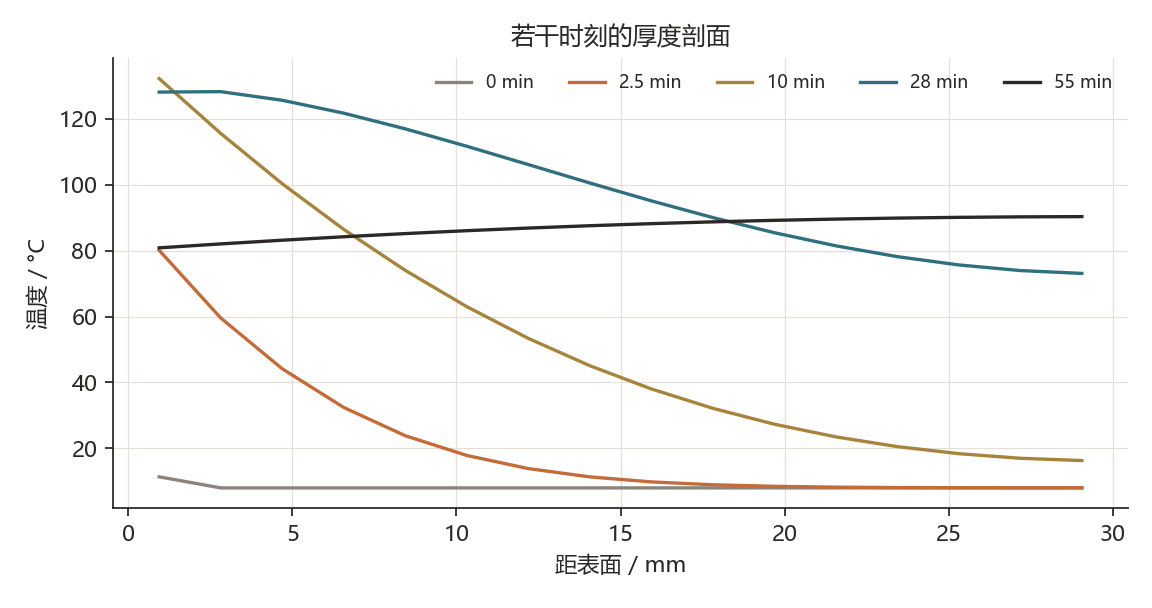
\includegraphics[width=0.9\textwidth]{paper/P_profiles.png}
\caption{0、2.5、10、28、55 min 的厚度剖面。2.5 min 时梯度集中在靠近表面的几个控制体。}
\end{figure}

\subsection{种子 7 的全部记录}
下表是 \texttt{demo\_seed7\_dual.csv} 的 414 行，记录间隔 8 s。表面温度是该步导热更新之后的值，冷点是更新之前十六个控制体的最低温度。估计冷点在观测器更新之后、导热更新之前写入。加热器温度不在这份 CSV 里。
\begin{longtable}{rrrrrrrr}
\caption{种子 7、对偶、肉糜 30 mm，全部记录}\\
\toprule
$t$ & 表面 & 冷点 & 估计 & $\alpha_m$ & 方差 & 加热 & 模式 \\
\midrule\endfirsthead
\toprule $t$ & 表面 & 冷点 & 估计 & $\alpha_m$ & 方差 & 加热 & 模式 \\\midrule\endhead
\bottomrule\endfoot
0 & 11.36 & 8.00 & -7.92 & 0.0000 & 0.640 & 1.000 & 品质 \\
8 & 21.45 & 8.00 & -7.79 & 0.0000 & 0.640 & 1.000 & 品质 \\
16 & 28.67 & 8.00 & -7.61 & 0.0000 & 0.640 & 1.000 & 品质 \\
24 & 34.43 & 8.00 & -7.39 & 0.0000 & 0.640 & 1.000 & 品质 \\
32 & 39.30 & 8.00 & -7.14 & 0.0000 & 0.640 & 1.000 & 品质 \\
40 & 43.55 & 8.00 & -6.86 & 0.0000 & 0.640 & 1.000 & 品质 \\
48 & 47.35 & 8.00 & -6.57 & 0.0000 & 0.640 & 1.000 & 品质 \\
56 & 50.80 & 8.00 & -6.25 & 0.0000 & 0.640 & 1.000 & 品质 \\
64 & 53.97 & 8.00 & -5.92 & 0.0000 & 0.640 & 1.000 & 品质 \\
72 & 56.90 & 8.00 & -5.57 & 0.0000 & 0.640 & 1.000 & 品质 \\
80 & 59.64 & 8.00 & -5.21 & 0.0000 & 0.640 & 1.000 & 品质 \\
88 & 62.20 & 8.00 & -4.83 & 0.0000 & 0.640 & 1.000 & 品质 \\
96 & 64.63 & 8.00 & -4.45 & 0.0000 & 0.640 & 1.000 & 品质 \\
104 & 66.92 & 8.00 & -4.05 & 0.0000 & 0.640 & 1.000 & 品质 \\
112 & 69.10 & 8.00 & -3.64 & 0.0000 & 0.640 & 1.000 & 品质 \\
120 & 71.17 & 8.00 & -3.22 & 0.0000 & 0.640 & 1.000 & 品质 \\
128 & 73.16 & 8.00 & -2.79 & 0.0000 & 0.640 & 1.000 & 品质 \\
136 & 75.06 & 8.00 & -2.36 & 0.0000 & 0.640 & 1.000 & 品质 \\
144 & 76.88 & 8.01 & -1.91 & 0.0000 & 0.640 & 1.000 & 品质 \\
152 & 80.10 & 8.01 & -1.45 & 0.0000 & 0.640 & 1.000 & 探针 \\
160 & 83.91 & 8.01 & -0.98 & 0.0000 & 0.640 & 1.000 & 探针 \\
168 & 87.12 & 8.02 & -0.49 & 0.0000 & 0.640 & 1.000 & 探针 \\
176 & 87.00 & 8.03 & 0.01 & 0.0000 & 0.640 & 1.000 & 探针 \\
184 & 87.57 & 8.04 & 0.51 & 0.0000 & 0.640 & 1.000 & 探针 \\
192 & 88.60 & 8.05 & 0.99 & 0.0000 & 0.224 & 1.000 & 品质 \\
200 & 89.85 & 8.06 & 1.41 & 0.0000 & 0.224 & 1.000 & 品质 \\
208 & 91.09 & 8.08 & 1.84 & 0.0000 & 0.224 & 1.000 & 品质 \\
216 & 92.31 & 8.10 & 2.28 & 0.0000 & 0.224 & 1.000 & 品质 \\
224 & 93.52 & 8.13 & 2.71 & 0.0000 & 0.224 & 1.000 & 品质 \\
232 & 94.70 & 8.16 & 3.15 & 0.0000 & 0.224 & 1.000 & 品质 \\
240 & 95.87 & 8.19 & 3.60 & 0.0000 & 0.224 & 1.000 & 品质 \\
248 & 97.01 & 8.23 & 4.05 & 0.0000 & 0.224 & 1.000 & 品质 \\
256 & 98.14 & 8.28 & 4.50 & 0.0000 & 0.224 & 1.000 & 品质 \\
264 & 99.24 & 8.33 & 4.95 & 0.0000 & 0.224 & 1.000 & 品质 \\
272 & 100.33 & 8.38 & 5.41 & 0.0000 & 0.224 & 1.000 & 品质 \\
280 & 101.39 & 8.44 & 5.87 & 0.0000 & 0.224 & 1.000 & 品质 \\
288 & 102.43 & 8.51 & 6.33 & 0.0000 & 0.224 & 1.000 & 品质 \\
296 & 103.45 & 8.58 & 6.80 & 0.0000 & 0.224 & 1.000 & 品质 \\
304 & 104.46 & 8.66 & 7.27 & 0.0000 & 0.224 & 1.000 & 品质 \\
312 & 105.44 & 8.75 & 7.74 & 0.0000 & 0.224 & 1.000 & 品质 \\
320 & 106.41 & 8.84 & 8.21 & 0.0000 & 0.224 & 1.000 & 品质 \\
328 & 107.36 & 8.94 & 8.69 & 0.0000 & 0.224 & 1.000 & 品质 \\
336 & 108.29 & 9.05 & 9.17 & 0.0000 & 0.224 & 1.000 & 品质 \\
344 & 109.21 & 9.16 & 9.65 & 0.0000 & 0.224 & 1.000 & 品质 \\
352 & 110.11 & 9.28 & 10.13 & 0.0000 & 0.224 & 1.000 & 品质 \\
360 & 111.00 & 9.40 & 10.62 & 0.0000 & 0.224 & 1.000 & 品质 \\
368 & 111.87 & 9.54 & 11.10 & 0.0000 & 0.224 & 1.000 & 品质 \\
376 & 112.72 & 9.68 & 11.59 & 0.0000 & 0.224 & 1.000 & 品质 \\
384 & 113.56 & 9.83 & 12.08 & 0.0000 & 0.224 & 1.000 & 品质 \\
392 & 114.39 & 9.98 & 12.58 & 0.0000 & 0.224 & 1.000 & 品质 \\
400 & 115.21 & 10.14 & 13.07 & 0.0000 & 0.224 & 1.000 & 品质 \\
408 & 116.01 & 10.31 & 13.56 & 0.0000 & 0.224 & 1.000 & 品质 \\
416 & 116.80 & 10.49 & 14.06 & 0.0000 & 0.224 & 1.000 & 品质 \\
424 & 117.58 & 10.67 & 14.56 & 0.0000 & 0.224 & 1.000 & 品质 \\
432 & 118.34 & 10.86 & 15.06 & 0.0000 & 0.224 & 1.000 & 品质 \\
440 & 119.10 & 11.05 & 15.56 & 0.0000 & 0.224 & 1.000 & 品质 \\
448 & 119.84 & 11.26 & 16.06 & 0.0000 & 0.224 & 1.000 & 品质 \\
456 & 120.57 & 11.47 & 16.56 & 0.0000 & 0.224 & 1.000 & 品质 \\
464 & 121.29 & 11.68 & 17.07 & 0.0000 & 0.224 & 1.000 & 品质 \\
472 & 122.01 & 11.90 & 17.57 & 0.0000 & 0.224 & 1.000 & 品质 \\
480 & 122.71 & 12.13 & 18.08 & 0.0000 & 0.224 & 1.000 & 品质 \\
488 & 123.40 & 12.36 & 18.59 & 0.0000 & 0.224 & 1.000 & 品质 \\
496 & 124.08 & 12.60 & 19.10 & 0.0000 & 0.224 & 1.000 & 品质 \\
504 & 124.76 & 12.85 & 19.61 & 0.0000 & 0.224 & 1.000 & 品质 \\
512 & 125.42 & 13.10 & 20.12 & 0.0000 & 0.224 & 1.000 & 品质 \\
520 & 126.08 & 13.36 & 20.63 & 0.0000 & 0.224 & 1.000 & 品质 \\
528 & 126.73 & 13.62 & 21.14 & 0.0000 & 0.224 & 1.000 & 品质 \\
536 & 127.37 & 13.89 & 21.65 & 0.0000 & 0.224 & 1.000 & 品质 \\
544 & 128.00 & 14.16 & 22.16 & 0.0000 & 0.224 & 1.000 & 品质 \\
552 & 128.63 & 14.44 & 22.67 & 0.0000 & 0.224 & 1.000 & 品质 \\
560 & 129.24 & 14.73 & 23.18 & 0.0000 & 0.224 & 1.000 & 品质 \\
568 & 129.85 & 15.02 & 23.70 & 0.0000 & 0.224 & 1.000 & 品质 \\
576 & 130.45 & 15.31 & 24.21 & 0.0000 & 0.224 & 1.000 & 品质 \\
584 & 131.05 & 15.61 & 24.73 & 0.0000 & 0.224 & 1.000 & 品质 \\
592 & 131.64 & 15.91 & 25.24 & 0.0000 & 0.224 & 1.000 & 品质 \\
600 & 132.22 & 16.22 & 25.76 & 0.0000 & 0.224 & 1.000 & 品质 \\
608 & 132.79 & 16.54 & 26.27 & 0.0000 & 0.224 & 1.000 & 品质 \\
616 & 133.36 & 16.85 & 26.79 & 0.0000 & 0.224 & 1.000 & 品质 \\
624 & 133.92 & 17.17 & 27.31 & 0.0000 & 0.224 & 1.000 & 品质 \\
632 & 134.48 & 17.50 & 27.82 & 0.0000 & 0.224 & 1.000 & 品质 \\
640 & 135.03 & 17.83 & 28.34 & 0.0000 & 0.224 & 1.000 & 品质 \\
648 & 135.57 & 18.17 & 28.86 & 0.0000 & 0.224 & 1.000 & 品质 \\
656 & 136.11 & 18.50 & 29.37 & 0.0000 & 0.224 & 1.000 & 品质 \\
664 & 136.64 & 18.85 & 29.89 & 0.0000 & 0.224 & 1.000 & 品质 \\
672 & 137.17 & 19.19 & 30.41 & 0.0000 & 0.224 & 1.000 & 品质 \\
680 & 137.69 & 19.54 & 30.93 & 0.0000 & 0.224 & 1.000 & 品质 \\
688 & 138.21 & 19.89 & 31.44 & 0.0000 & 0.224 & 1.000 & 品质 \\
696 & 138.72 & 20.25 & 31.96 & 0.0000 & 0.224 & 1.000 & 品质 \\
704 & 139.23 & 20.61 & 32.48 & 0.0000 & 0.224 & 1.000 & 品质 \\
712 & 139.73 & 20.97 & 32.99 & 0.0000 & 0.224 & 1.000 & 品质 \\
720 & 140.22 & 21.34 & 33.51 & 0.0000 & 0.224 & 1.000 & 品质 \\
728 & 140.72 & 21.71 & 34.03 & 0.0000 & 0.224 & 1.000 & 品质 \\
736 & 141.20 & 22.08 & 34.54 & 0.0000 & 0.224 & 1.000 & 品质 \\
744 & 141.69 & 22.46 & 35.06 & 0.0000 & 0.224 & 1.000 & 品质 \\
752 & 142.16 & 22.84 & 35.58 & 0.0000 & 0.224 & 1.000 & 品质 \\
760 & 142.64 & 23.22 & 36.09 & 0.0000 & 0.224 & 1.000 & 品质 \\
768 & 143.11 & 23.60 & 36.61 & 0.0000 & 0.224 & 1.000 & 品质 \\
776 & 143.57 & 23.99 & 37.12 & 0.0000 & 0.224 & 1.000 & 品质 \\
784 & 144.03 & 24.38 & 37.64 & 0.0000 & 0.224 & 1.000 & 品质 \\
792 & 144.49 & 24.77 & 38.15 & 0.0000 & 0.224 & 1.000 & 品质 \\
800 & 144.95 & 25.16 & 38.67 & 0.0000 & 0.224 & 1.000 & 品质 \\
808 & 145.40 & 25.56 & 39.18 & 0.0000 & 0.224 & 1.000 & 品质 \\
816 & 145.84 & 25.96 & 39.70 & 0.0000 & 0.224 & 1.000 & 品质 \\
824 & 146.28 & 26.36 & 40.21 & 0.0000 & 0.224 & 1.000 & 品质 \\
832 & 146.72 & 26.76 & 40.73 & 0.0000 & 0.224 & 1.000 & 品质 \\
840 & 147.16 & 27.17 & 41.24 & 0.0000 & 0.224 & 1.000 & 品质 \\
848 & 147.59 & 27.57 & 41.75 & 0.0001 & 0.224 & 1.000 & 品质 \\
856 & 148.02 & 27.98 & 42.26 & 0.0001 & 0.224 & 1.000 & 品质 \\
864 & 148.44 & 28.39 & 42.78 & 0.0001 & 0.224 & 1.000 & 品质 \\
872 & 148.86 & 28.81 & 43.29 & 0.0001 & 0.224 & 1.000 & 品质 \\
880 & 149.28 & 29.22 & 43.80 & 0.0001 & 0.224 & 1.000 & 品质 \\
888 & 149.70 & 29.64 & 44.31 & 0.0001 & 0.224 & 1.000 & 品质 \\
896 & 150.11 & 30.06 & 44.82 & 0.0001 & 0.224 & 1.000 & 品质 \\
904 & 150.52 & 30.48 & 45.33 & 0.0001 & 0.224 & 1.000 & 品质 \\
912 & 150.93 & 30.90 & 45.84 & 0.0001 & 0.224 & 1.000 & 品质 \\
920 & 151.33 & 31.32 & 46.35 & 0.0001 & 0.224 & 1.000 & 品质 \\
928 & 151.73 & 31.74 & 46.86 & 0.0001 & 0.224 & 1.000 & 品质 \\
936 & 152.13 & 32.17 & 47.36 & 0.0001 & 0.224 & 1.000 & 品质 \\
944 & 152.52 & 32.60 & 47.87 & 0.0001 & 0.224 & 1.000 & 品质 \\
952 & 152.91 & 33.02 & 48.38 & 0.0001 & 0.224 & 1.000 & 品质 \\
960 & 153.30 & 33.45 & 48.88 & 0.0002 & 0.224 & 1.000 & 品质 \\
968 & 153.69 & 33.88 & 49.39 & 0.0002 & 0.224 & 1.000 & 品质 \\
976 & 154.08 & 34.32 & 49.89 & 0.0002 & 0.224 & 1.000 & 品质 \\
984 & 154.46 & 34.75 & 50.40 & 0.0002 & 0.224 & 1.000 & 品质 \\
992 & 154.84 & 35.18 & 50.90 & 0.0002 & 0.224 & 1.000 & 品质 \\
1000 & 155.21 & 35.62 & 51.40 & 0.0003 & 0.224 & 1.000 & 品质 \\
1008 & 155.59 & 36.05 & 51.91 & 0.0003 & 0.224 & 1.000 & 品质 \\
1016 & 155.96 & 36.49 & 52.41 & 0.0003 & 0.224 & 1.000 & 品质 \\
1024 & 156.33 & 36.93 & 52.91 & 0.0003 & 0.224 & 1.000 & 品质 \\
1032 & 156.70 & 37.37 & 53.41 & 0.0004 & 0.224 & 1.000 & 品质 \\
1040 & 157.06 & 37.81 & 53.91 & 0.0004 & 0.224 & 1.000 & 品质 \\
1048 & 157.43 & 38.25 & 54.41 & 0.0005 & 0.224 & 1.000 & 品质 \\
1056 & 157.79 & 38.69 & 54.91 & 0.0005 & 0.224 & 1.000 & 品质 \\
1064 & 158.15 & 39.13 & 55.40 & 0.0006 & 0.224 & 1.000 & 品质 \\
1072 & 158.51 & 39.57 & 55.90 & 0.0006 & 0.224 & 1.000 & 品质 \\
1080 & 158.86 & 40.01 & 56.40 & 0.0007 & 0.224 & 1.000 & 品质 \\
1088 & 159.21 & 40.46 & 56.89 & 0.0008 & 0.224 & 1.000 & 品质 \\
1096 & 159.57 & 40.90 & 57.39 & 0.0008 & 0.224 & 1.000 & 品质 \\
1104 & 159.91 & 41.35 & 57.88 & 0.0009 & 0.224 & 1.000 & 品质 \\
1112 & 160.26 & 41.79 & 58.38 & 0.0010 & 0.224 & 1.000 & 品质 \\
1120 & 160.61 & 42.24 & 58.87 & 0.0011 & 0.224 & 1.000 & 品质 \\
1128 & 160.95 & 42.68 & 59.36 & 0.0012 & 0.224 & 1.000 & 品质 \\
1136 & 161.29 & 43.13 & 59.86 & 0.0014 & 0.224 & 1.000 & 品质 \\
1144 & 161.63 & 43.58 & 60.35 & 0.0015 & 0.224 & 1.000 & 品质 \\
1152 & 161.97 & 44.03 & 60.84 & 0.0017 & 0.224 & 1.000 & 品质 \\
1160 & 162.31 & 44.47 & 61.33 & 0.0019 & 0.224 & 1.000 & 品质 \\
1168 & 162.64 & 44.92 & 61.81 & 0.0021 & 0.224 & 1.000 & 品质 \\
1176 & 162.98 & 45.37 & 62.30 & 0.0023 & 0.224 & 1.000 & 品质 \\
1184 & 163.31 & 45.82 & 62.79 & 0.0025 & 0.224 & 1.000 & 品质 \\
1192 & 163.64 & 46.27 & 63.28 & 0.0028 & 0.224 & 1.000 & 品质 \\
1200 & 163.97 & 46.72 & 63.76 & 0.0031 & 0.224 & 1.000 & 品质 \\
1208 & 164.29 & 47.17 & 64.25 & 0.0034 & 0.224 & 1.000 & 品质 \\
1216 & 164.62 & 47.62 & 64.73 & 0.0038 & 0.224 & 1.000 & 品质 \\
1224 & 164.94 & 48.07 & 65.22 & 0.0042 & 0.224 & 1.000 & 品质 \\
1232 & 165.27 & 48.52 & 65.70 & 0.0047 & 0.224 & 1.000 & 品质 \\
1240 & 165.59 & 48.97 & 66.18 & 0.0052 & 0.224 & 1.000 & 品质 \\
1248 & 165.81 & 49.42 & 66.66 & 0.0057 & 0.224 & 0.986 & 品质 \\
1256 & 165.89 & 49.87 & 67.14 & 0.0063 & 0.224 & 0.970 & 品质 \\
1264 & 165.87 & 50.32 & 67.62 & 0.0070 & 0.224 & 0.954 & 品质 \\
1272 & 165.76 & 50.77 & 68.09 & 0.0078 & 0.224 & 0.938 & 品质 \\
1280 & 165.58 & 51.22 & 68.56 & 0.0086 & 0.224 & 0.922 & 品质 \\
1288 & 165.35 & 51.67 & 69.03 & 0.0096 & 0.224 & 0.907 & 品质 \\
1296 & 165.05 & 52.12 & 69.50 & 0.0106 & 0.224 & 0.891 & 品质 \\
1304 & 164.71 & 52.57 & 69.96 & 0.0118 & 0.224 & 0.876 & 品质 \\
1312 & 164.32 & 53.02 & 70.42 & 0.0130 & 0.224 & 0.861 & 品质 \\
1320 & 163.89 & 53.47 & 70.87 & 0.0144 & 0.224 & 0.845 & 品质 \\
1328 & 163.43 & 53.92 & 71.32 & 0.0160 & 0.224 & 0.830 & 品质 \\
1336 & 162.93 & 54.37 & 71.76 & 0.0177 & 0.224 & 0.816 & 品质 \\
1344 & 162.40 & 54.82 & 72.20 & 0.0196 & 0.224 & 0.801 & 品质 \\
1352 & 161.84 & 55.27 & 72.64 & 0.0217 & 0.224 & 0.787 & 品质 \\
1360 & 161.26 & 55.72 & 73.07 & 0.0241 & 0.224 & 0.772 & 品质 \\
1368 & 160.65 & 56.17 & 73.49 & 0.0267 & 0.224 & 0.758 & 品质 \\
1376 & 160.02 & 56.62 & 73.91 & 0.0295 & 0.224 & 0.744 & 品质 \\
1384 & 159.36 & 57.07 & 74.33 & 0.0327 & 0.224 & 0.730 & 品质 \\
1392 & 158.69 & 57.52 & 74.74 & 0.0362 & 0.224 & 0.716 & 品质 \\
1400 & 158.00 & 57.97 & 75.14 & 0.0401 & 0.224 & 0.703 & 品质 \\
1408 & 157.29 & 58.41 & 75.54 & 0.0443 & 0.224 & 0.690 & 品质 \\
1416 & 156.57 & 58.86 & 75.94 & 0.0490 & 0.224 & 0.677 & 品质 \\
1424 & 155.84 & 59.31 & 76.32 & 0.0542 & 0.224 & 0.664 & 品质 \\
1432 & 155.09 & 59.76 & 76.71 & 0.0599 & 0.224 & 0.651 & 品质 \\
1440 & 154.33 & 60.20 & 77.08 & 0.0662 & 0.224 & 0.638 & 品质 \\
1448 & 153.56 & 60.65 & 77.46 & 0.0732 & 0.224 & 0.626 & 品质 \\
1456 & 152.78 & 61.09 & 77.82 & 0.0808 & 0.224 & 0.614 & 品质 \\
1464 & 151.99 & 61.54 & 78.18 & 0.0892 & 0.224 & 0.602 & 品质 \\
1472 & 151.19 & 61.98 & 78.54 & 0.0983 & 0.224 & 0.590 & 品质 \\
1480 & 150.39 & 62.43 & 78.89 & 0.1084 & 0.224 & 0.578 & 品质 \\
1488 & 149.58 & 62.87 & 79.24 & 0.1194 & 0.224 & 0.567 & 品质 \\
1496 & 148.76 & 63.31 & 79.57 & 0.1315 & 0.224 & 0.555 & 品质 \\
1504 & 147.94 & 63.75 & 79.91 & 0.1446 & 0.224 & 0.544 & 品质 \\
1512 & 147.11 & 64.19 & 80.23 & 0.1589 & 0.224 & 0.533 & 品质 \\
1520 & 146.29 & 64.63 & 80.56 & 0.1744 & 0.224 & 0.523 & 品质 \\
1528 & 145.46 & 65.07 & 80.87 & 0.1913 & 0.224 & 0.512 & 品质 \\
1536 & 144.62 & 65.50 & 81.18 & 0.2095 & 0.224 & 0.502 & 品质 \\
1544 & 143.79 & 65.94 & 81.49 & 0.2292 & 0.224 & 0.491 & 品质 \\
1552 & 142.95 & 66.37 & 81.79 & 0.2504 & 0.224 & 0.482 & 品质 \\
1560 & 142.12 & 66.80 & 82.08 & 0.2731 & 0.224 & 0.472 & 品质 \\
1568 & 141.28 & 67.23 & 82.37 & 0.2973 & 0.224 & 0.462 & 品质 \\
1576 & 140.45 & 67.66 & 82.65 & 0.3232 & 0.224 & 0.453 & 品质 \\
1584 & 139.61 & 68.08 & 82.93 & 0.3506 & 0.224 & 0.443 & 品质 \\
1592 & 138.78 & 68.50 & 83.20 & 0.3795 & 0.224 & 0.434 & 品质 \\
1600 & 137.95 & 68.93 & 83.47 & 0.4099 & 0.224 & 0.425 & 品质 \\
1608 & 137.12 & 69.34 & 83.73 & 0.4416 & 0.224 & 0.417 & 品质 \\
1616 & 136.29 & 69.76 & 83.99 & 0.4746 & 0.224 & 0.408 & 品质 \\
1624 & 135.47 & 70.18 & 84.24 & 0.5087 & 0.224 & 0.400 & 品质 \\
1632 & 134.64 & 70.59 & 84.49 & 0.5436 & 0.224 & 0.392 & 品质 \\
1640 & 133.83 & 71.00 & 84.73 & 0.5791 & 0.224 & 0.384 & 品质 \\
1648 & 133.01 & 71.40 & 84.96 & 0.6149 & 0.224 & 0.376 & 品质 \\
1656 & 132.21 & 71.80 & 85.19 & 0.6507 & 0.224 & 0.368 & 品质 \\
1664 & 131.40 & 72.21 & 85.42 & 0.6862 & 0.224 & 0.360 & 品质 \\
1672 & 130.60 & 72.60 & 85.64 & 0.7209 & 0.224 & 0.353 & 品质 \\
1680 & 128.12 & 73.00 & 85.85 & 0.7546 & 0.224 & 0.150 & 保持 \\
1688 & 125.82 & 73.39 & 86.05 & 0.7868 & 0.224 & 0.150 & 保持 \\
1696 & 123.96 & 73.78 & 86.24 & 0.8172 & 0.224 & 0.150 & 保持 \\
1704 & 122.34 & 74.16 & 86.42 & 0.8455 & 0.224 & 0.150 & 保持 \\
1712 & 120.91 & 74.54 & 86.59 & 0.8714 & 0.224 & 0.150 & 保持 \\
1720 & 119.60 & 74.92 & 86.76 & 0.8948 & 0.224 & 0.150 & 保持 \\
1728 & 118.40 & 75.30 & 86.91 & 0.9154 & 0.224 & 0.150 & 保持 \\
1736 & 117.28 & 75.67 & 87.06 & 0.9334 & 0.224 & 0.150 & 保持 \\
1744 & 116.24 & 76.03 & 87.21 & 0.9486 & 0.224 & 0.150 & 保持 \\
1752 & 115.25 & 76.40 & 87.35 & 0.9612 & 0.224 & 0.150 & 保持 \\
1760 & 114.32 & 76.76 & 87.48 & 0.9715 & 0.224 & 0.150 & 保持 \\
1768 & 113.43 & 77.12 & 87.61 & 0.9795 & 0.224 & 0.150 & 保持 \\
1776 & 112.59 & 77.47 & 87.73 & 0.9857 & 0.224 & 0.150 & 保持 \\
1784 & 111.79 & 77.82 & 87.85 & 0.9904 & 0.224 & 0.150 & 保持 \\
1792 & 111.02 & 78.16 & 87.96 & 0.9937 & 0.224 & 0.150 & 保持 \\
1800 & 110.28 & 78.50 & 88.07 & 0.9960 & 0.224 & 0.150 & 保持 \\
1808 & 109.57 & 78.84 & 88.18 & 0.9976 & 0.224 & 0.150 & 保持 \\
1816 & 108.89 & 79.17 & 88.28 & 0.9986 & 0.224 & 0.150 & 保持 \\
1824 & 108.23 & 79.50 & 88.38 & 0.9992 & 0.224 & 0.150 & 保持 \\
1832 & 107.60 & 79.82 & 88.14 & 0.9996 & 0.224 & 0.150 & 保持 \\
1840 & 106.99 & 80.14 & 87.55 & 0.9998 & 0.224 & 0.150 & 保持 \\
1848 & 106.39 & 80.46 & 87.01 & 0.9999 & 0.224 & 0.150 & 保持 \\
1856 & 105.82 & 80.77 & 86.03 & 1.0000 & 0.224 & 0.150 & 保持 \\
1864 & 105.27 & 81.08 & 85.94 & 1.0000 & 0.224 & 0.150 & 保持 \\
1872 & 104.73 & 81.38 & 85.14 & 1.0000 & 0.224 & 0.150 & 保持 \\
1880 & 104.22 & 81.67 & 84.90 & 1.0000 & 0.224 & 0.150 & 保持 \\
1888 & 103.71 & 81.97 & 84.04 & 1.0000 & 0.224 & 0.150 & 保持 \\
1896 & 103.22 & 82.25 & 83.45 & 1.0000 & 0.224 & 0.150 & 保持 \\
1904 & 102.75 & 82.54 & 83.08 & 1.0000 & 0.224 & 0.150 & 保持 \\
1912 & 102.29 & 82.81 & 83.12 & 1.0000 & 0.224 & 0.150 & 保持 \\
1920 & 101.84 & 83.09 & 82.39 & 1.0000 & 0.224 & 0.150 & 保持 \\
1928 & 101.40 & 83.35 & 81.59 & 1.0000 & 0.224 & 0.150 & 保持 \\
1936 & 100.98 & 83.62 & 81.46 & 1.0000 & 0.224 & 0.150 & 保持 \\
1944 & 100.57 & 83.87 & 80.87 & 1.0000 & 0.224 & 0.150 & 保持 \\
1952 & 100.16 & 84.13 & 80.87 & 1.0000 & 0.224 & 0.150 & 保持 \\
1960 & 99.77 & 84.37 & 80.04 & 1.0000 & 0.224 & 0.150 & 保持 \\
1968 & 99.39 & 84.62 & 80.04 & 1.0000 & 0.224 & 0.150 & 保持 \\
1976 & 99.02 & 84.85 & 79.41 & 1.0000 & 0.224 & 0.150 & 保持 \\
1984 & 98.66 & 85.09 & 79.13 & 1.0000 & 0.224 & 0.150 & 保持 \\
1992 & 98.30 & 85.31 & 78.55 & 1.0000 & 0.224 & 0.150 & 保持 \\
2000 & 97.96 & 85.54 & 78.36 & 1.0000 & 0.224 & 0.150 & 保持 \\
2008 & 97.62 & 85.75 & 77.93 & 1.0000 & 0.224 & 0.150 & 保持 \\
2016 & 97.29 & 85.97 & 77.78 & 1.0000 & 0.224 & 0.150 & 保持 \\
2024 & 96.97 & 86.17 & 77.27 & 1.0000 & 0.224 & 0.150 & 保持 \\
2032 & 96.66 & 86.38 & 76.85 & 1.0000 & 0.224 & 0.150 & 保持 \\
2040 & 96.35 & 86.58 & 76.47 & 1.0000 & 0.224 & 0.150 & 保持 \\
2048 & 96.05 & 86.77 & 76.40 & 1.0000 & 0.224 & 0.150 & 保持 \\
2056 & 95.76 & 86.96 & 76.00 & 1.0000 & 0.224 & 0.150 & 保持 \\
2064 & 95.48 & 87.14 & 75.65 & 1.0000 & 0.224 & 0.150 & 保持 \\
2072 & 95.20 & 87.32 & 75.27 & 1.0000 & 0.224 & 0.150 & 保持 \\
2080 & 94.92 & 87.50 & 75.37 & 1.0000 & 0.224 & 0.150 & 保持 \\
2088 & 94.66 & 87.67 & 75.12 & 1.0000 & 0.224 & 0.150 & 保持 \\
2096 & 94.39 & 87.83 & 74.68 & 1.0000 & 0.224 & 0.150 & 保持 \\
2104 & 94.14 & 88.00 & 74.36 & 1.0000 & 0.224 & 0.150 & 保持 \\
2112 & 93.89 & 88.15 & 74.45 & 1.0000 & 0.224 & 0.150 & 保持 \\
2120 & 93.64 & 88.31 & 73.99 & 1.0000 & 0.224 & 0.150 & 保持 \\
2128 & 93.41 & 88.46 & 73.65 & 1.0000 & 0.224 & 0.150 & 保持 \\
2136 & 93.17 & 88.60 & 73.46 & 1.0000 & 0.224 & 0.150 & 保持 \\
2144 & 92.94 & 88.74 & 73.54 & 1.0000 & 0.224 & 0.150 & 保持 \\
2152 & 92.72 & 88.88 & 72.98 & 1.0000 & 0.224 & 0.150 & 保持 \\
2160 & 92.50 & 89.01 & 72.69 & 1.0000 & 0.224 & 0.150 & 保持 \\
2168 & 92.28 & 89.14 & 72.43 & 1.0000 & 0.224 & 0.150 & 保持 \\
2176 & 92.07 & 89.27 & 72.51 & 1.0000 & 0.224 & 0.150 & 保持 \\
2184 & 91.86 & 89.39 & 72.42 & 1.0000 & 0.224 & 0.150 & 保持 \\
2192 & 91.66 & 89.51 & 72.00 & 1.0000 & 0.224 & 0.150 & 保持 \\
2200 & 91.46 & 89.63 & 71.79 & 1.0000 & 0.224 & 0.150 & 保持 \\
2208 & 91.27 & 89.74 & 71.55 & 1.0000 & 0.224 & 0.150 & 保持 \\
2216 & 91.08 & 89.85 & 71.45 & 1.0000 & 0.224 & 0.150 & 保持 \\
2224 & 90.89 & 89.95 & 71.25 & 1.0000 & 0.224 & 0.150 & 保持 \\
2232 & 90.71 & 90.05 & 71.02 & 1.0000 & 0.224 & 0.150 & 保持 \\
2240 & 90.53 & 90.15 & 71.08 & 1.0000 & 0.224 & 0.150 & 保持 \\
2248 & 90.35 & 90.25 & 70.77 & 1.0000 & 0.224 & 0.150 & 保持 \\
2256 & 90.18 & 90.22 & 70.44 & 1.0000 & 0.224 & 0.150 & 保持 \\
2264 & 90.01 & 90.05 & 70.31 & 1.0000 & 0.224 & 0.150 & 保持 \\
2272 & 89.85 & 89.89 & 70.04 & 1.0000 & 0.224 & 0.150 & 保持 \\
2280 & 89.68 & 89.72 & 69.93 & 1.0000 & 0.224 & 0.150 & 保持 \\
2288 & 89.52 & 89.56 & 69.73 & 1.0000 & 0.224 & 0.150 & 保持 \\
2296 & 89.37 & 89.40 & 69.51 & 1.0000 & 0.224 & 0.150 & 保持 \\
2304 & 89.21 & 89.25 & 69.60 & 1.0000 & 0.224 & 0.150 & 保持 \\
2312 & 89.06 & 89.10 & 69.14 & 1.0000 & 0.224 & 0.150 & 保持 \\
2320 & 88.91 & 88.95 & 69.06 & 1.0000 & 0.224 & 0.150 & 保持 \\
2328 & 88.77 & 88.80 & 68.95 & 1.0000 & 0.224 & 0.150 & 保持 \\
2336 & 88.63 & 88.66 & 68.80 & 1.0000 & 0.224 & 0.150 & 保持 \\
2344 & 88.49 & 88.52 & 68.76 & 1.0000 & 0.224 & 0.150 & 保持 \\
2352 & 88.35 & 88.38 & 68.42 & 1.0000 & 0.224 & 0.150 & 保持 \\
2360 & 88.21 & 88.25 & 68.52 & 1.0000 & 0.224 & 0.150 & 保持 \\
2368 & 88.08 & 88.11 & 68.51 & 1.0000 & 0.224 & 0.150 & 保持 \\
2376 & 87.95 & 87.98 & 68.32 & 1.0000 & 0.224 & 0.150 & 保持 \\
2384 & 87.82 & 87.86 & 68.00 & 1.0000 & 0.224 & 0.150 & 保持 \\
2392 & 87.70 & 87.73 & 68.00 & 1.0000 & 0.224 & 0.150 & 保持 \\
2400 & 87.57 & 87.61 & 67.98 & 1.0000 & 0.224 & 0.150 & 保持 \\
2408 & 87.45 & 87.48 & 67.84 & 1.0000 & 0.224 & 0.150 & 保持 \\
2416 & 87.33 & 87.36 & 67.59 & 1.0000 & 0.224 & 0.150 & 保持 \\
2424 & 87.22 & 87.25 & 67.37 & 1.0000 & 0.224 & 0.150 & 保持 \\
2432 & 87.10 & 87.13 & 67.44 & 1.0000 & 0.224 & 0.150 & 保持 \\
2440 & 86.99 & 87.02 & 67.25 & 1.0000 & 0.224 & 0.150 & 保持 \\
2448 & 86.88 & 86.91 & 66.97 & 1.0000 & 0.224 & 0.150 & 保持 \\
2456 & 86.77 & 86.80 & 66.95 & 1.0000 & 0.224 & 0.150 & 保持 \\
2464 & 86.66 & 86.69 & 66.99 & 1.0000 & 0.224 & 0.150 & 保持 \\
2472 & 86.56 & 86.58 & 67.09 & 1.0000 & 0.224 & 0.150 & 保持 \\
2480 & 86.45 & 86.48 & 66.74 & 1.0000 & 0.224 & 0.150 & 保持 \\
2488 & 86.35 & 86.38 & 66.70 & 1.0000 & 0.224 & 0.150 & 保持 \\
2496 & 86.25 & 86.28 & 66.35 & 1.0000 & 0.224 & 0.150 & 保持 \\
2504 & 86.15 & 86.18 & 66.29 & 1.0000 & 0.224 & 0.150 & 保持 \\
2512 & 86.06 & 86.08 & 66.39 & 1.0000 & 0.224 & 0.150 & 保持 \\
2520 & 85.96 & 85.99 & 66.12 & 1.0000 & 0.224 & 0.150 & 保持 \\
2528 & 85.87 & 85.89 & 66.04 & 1.0000 & 0.224 & 0.150 & 保持 \\
2536 & 85.78 & 85.80 & 65.92 & 1.0000 & 0.224 & 0.150 & 保持 \\
2544 & 85.69 & 85.71 & 65.91 & 1.0000 & 0.224 & 0.150 & 保持 \\
2552 & 85.60 & 85.62 & 65.85 & 1.0000 & 0.224 & 0.150 & 保持 \\
2560 & 85.51 & 85.53 & 65.85 & 1.0000 & 0.224 & 0.150 & 保持 \\
2568 & 85.42 & 85.44 & 65.75 & 1.0000 & 0.224 & 0.150 & 保持 \\
2576 & 85.34 & 85.36 & 65.85 & 1.0000 & 0.224 & 0.150 & 保持 \\
2584 & 85.25 & 85.27 & 65.58 & 1.0000 & 0.224 & 0.150 & 保持 \\
2592 & 85.17 & 85.19 & 65.33 & 1.0000 & 0.224 & 0.150 & 保持 \\
2600 & 85.09 & 85.11 & 65.30 & 1.0000 & 0.224 & 0.150 & 保持 \\
2608 & 85.01 & 85.03 & 65.22 & 1.0000 & 0.224 & 0.150 & 保持 \\
2616 & 84.93 & 84.95 & 65.31 & 1.0000 & 0.224 & 0.150 & 保持 \\
2624 & 84.85 & 84.87 & 65.11 & 1.0000 & 0.224 & 0.150 & 保持 \\
2632 & 84.78 & 84.80 & 64.95 & 1.0000 & 0.224 & 0.150 & 保持 \\
2640 & 84.70 & 84.72 & 64.92 & 1.0000 & 0.224 & 0.150 & 保持 \\
2648 & 84.63 & 84.65 & 65.01 & 1.0000 & 0.224 & 0.150 & 保持 \\
2656 & 84.56 & 84.57 & 64.78 & 1.0000 & 0.224 & 0.150 & 保持 \\
2664 & 84.48 & 84.50 & 64.58 & 1.0000 & 0.224 & 0.150 & 保持 \\
2672 & 84.41 & 84.43 & 64.68 & 1.0000 & 0.224 & 0.150 & 保持 \\
2680 & 84.34 & 84.36 & 64.59 & 1.0000 & 0.224 & 0.150 & 保持 \\
2688 & 84.27 & 84.29 & 64.47 & 1.0000 & 0.224 & 0.150 & 保持 \\
2696 & 84.21 & 84.22 & 64.35 & 1.0000 & 0.224 & 0.150 & 保持 \\
2704 & 84.14 & 84.16 & 64.31 & 1.0000 & 0.224 & 0.150 & 保持 \\
2712 & 84.07 & 84.09 & 64.24 & 1.0000 & 0.224 & 0.150 & 保持 \\
2720 & 84.01 & 84.02 & 64.33 & 1.0000 & 0.224 & 0.150 & 保持 \\
2728 & 83.94 & 83.96 & 64.02 & 1.0000 & 0.224 & 0.150 & 保持 \\
2736 & 83.88 & 83.90 & 64.11 & 1.0000 & 0.224 & 0.150 & 保持 \\
2744 & 83.82 & 83.83 & 63.88 & 1.0000 & 0.224 & 0.150 & 保持 \\
2752 & 83.76 & 83.77 & 63.94 & 1.0000 & 0.224 & 0.150 & 保持 \\
2760 & 83.70 & 83.71 & 63.85 & 1.0000 & 0.224 & 0.150 & 保持 \\
2768 & 83.64 & 83.65 & 63.85 & 1.0000 & 0.224 & 0.150 & 保持 \\
2776 & 83.58 & 83.59 & 63.60 & 1.0000 & 0.224 & 0.150 & 保持 \\
2784 & 83.52 & 83.53 & 63.62 & 1.0000 & 0.224 & 0.150 & 保持 \\
2792 & 83.46 & 83.48 & 63.62 & 1.0000 & 0.224 & 0.150 & 保持 \\
2800 & 83.40 & 83.42 & 63.65 & 1.0000 & 0.224 & 0.150 & 保持 \\
2808 & 83.35 & 83.36 & 63.74 & 1.0000 & 0.224 & 0.150 & 保持 \\
2816 & 83.29 & 83.31 & 63.53 & 1.0000 & 0.224 & 0.150 & 保持 \\
2824 & 83.24 & 83.25 & 63.32 & 1.0000 & 0.224 & 0.150 & 保持 \\
2832 & 83.18 & 83.20 & 63.42 & 1.0000 & 0.224 & 0.150 & 保持 \\
2840 & 83.13 & 83.14 & 63.48 & 1.0000 & 0.224 & 0.150 & 保持 \\
2848 & 83.08 & 83.09 & 63.25 & 1.0000 & 0.224 & 0.150 & 保持 \\
2856 & 83.03 & 83.04 & 63.34 & 1.0000 & 0.224 & 0.150 & 保持 \\
2864 & 82.97 & 82.99 & 63.21 & 1.0000 & 0.224 & 0.150 & 保持 \\
2872 & 82.92 & 82.94 & 63.13 & 1.0000 & 0.224 & 0.150 & 保持 \\
2880 & 82.87 & 82.89 & 62.97 & 1.0000 & 0.224 & 0.150 & 保持 \\
2888 & 82.82 & 82.84 & 63.07 & 1.0000 & 0.224 & 0.150 & 保持 \\
2896 & 82.78 & 82.79 & 62.93 & 1.0000 & 0.224 & 0.150 & 保持 \\
2904 & 82.73 & 82.74 & 62.98 & 1.0000 & 0.224 & 0.150 & 保持 \\
2912 & 82.68 & 82.69 & 62.94 & 1.0000 & 0.224 & 0.150 & 保持 \\
2920 & 82.63 & 82.64 & 63.03 & 1.0000 & 0.224 & 0.150 & 保持 \\
2928 & 82.58 & 82.60 & 62.78 & 1.0000 & 0.224 & 0.150 & 保持 \\
2936 & 82.54 & 82.55 & 62.69 & 1.0000 & 0.224 & 0.150 & 保持 \\
2944 & 82.49 & 82.50 & 62.79 & 1.0000 & 0.224 & 0.150 & 保持 \\
2952 & 82.45 & 82.46 & 62.61 & 1.0000 & 0.224 & 0.150 & 保持 \\
2960 & 82.40 & 82.41 & 62.65 & 1.0000 & 0.224 & 0.150 & 保持 \\
2968 & 82.36 & 82.37 & 62.48 & 1.0000 & 0.224 & 0.150 & 保持 \\
2976 & 82.31 & 82.32 & 62.50 & 1.0000 & 0.224 & 0.150 & 保持 \\
2984 & 82.27 & 82.28 & 62.45 & 1.0000 & 0.224 & 0.150 & 保持 \\
2992 & 82.23 & 82.24 & 62.54 & 1.0000 & 0.224 & 0.150 & 保持 \\
3000 & 82.18 & 82.20 & 62.64 & 1.0000 & 0.224 & 0.150 & 保持 \\
3008 & 82.14 & 82.15 & 62.46 & 1.0000 & 0.224 & 0.150 & 保持 \\
3016 & 82.10 & 82.11 & 62.27 & 1.0000 & 0.224 & 0.150 & 保持 \\
3024 & 82.06 & 82.07 & 62.29 & 1.0000 & 0.224 & 0.150 & 保持 \\
3032 & 82.02 & 82.03 & 62.18 & 1.0000 & 0.224 & 0.150 & 保持 \\
3040 & 81.98 & 81.99 & 62.16 & 1.0000 & 0.224 & 0.150 & 保持 \\
3048 & 81.94 & 81.95 & 62.09 & 1.0000 & 0.224 & 0.150 & 保持 \\
3056 & 81.90 & 81.91 & 62.05 & 1.0000 & 0.224 & 0.150 & 保持 \\
3064 & 81.86 & 81.87 & 62.15 & 1.0000 & 0.224 & 0.150 & 保持 \\
3072 & 81.82 & 81.83 & 62.14 & 1.0000 & 0.224 & 0.150 & 保持 \\
3080 & 81.78 & 81.79 & 62.08 & 1.0000 & 0.224 & 0.150 & 保持 \\
3088 & 81.74 & 81.75 & 61.93 & 1.0000 & 0.224 & 0.150 & 保持 \\
3096 & 81.70 & 81.71 & 61.99 & 1.0000 & 0.224 & 0.150 & 保持 \\
3104 & 81.67 & 81.68 & 61.77 & 1.0000 & 0.224 & 0.150 & 保持 \\
3112 & 81.63 & 81.64 & 61.76 & 1.0000 & 0.224 & 0.150 & 保持 \\
3120 & 81.59 & 81.60 & 61.66 & 1.0000 & 0.224 & 0.150 & 保持 \\
3128 & 81.56 & 81.57 & 61.60 & 1.0000 & 0.224 & 0.150 & 保持 \\
3136 & 81.52 & 81.53 & 61.70 & 1.0000 & 0.224 & 0.150 & 保持 \\
3144 & 81.48 & 81.49 & 61.77 & 1.0000 & 0.224 & 0.150 & 保持 \\
3152 & 81.45 & 81.46 & 61.46 & 1.0000 & 0.224 & 0.150 & 保持 \\
3160 & 81.41 & 81.42 & 61.56 & 1.0000 & 0.224 & 0.150 & 保持 \\
3168 & 81.38 & 81.39 & 61.49 & 1.0000 & 0.224 & 0.150 & 保持 \\
3176 & 81.34 & 81.35 & 61.58 & 1.0000 & 0.224 & 0.150 & 保持 \\
3184 & 81.31 & 81.32 & 61.48 & 1.0000 & 0.224 & 0.150 & 保持 \\
3192 & 81.27 & 81.28 & 61.57 & 1.0000 & 0.224 & 0.150 & 保持 \\
3200 & 81.24 & 81.25 & 61.67 & 1.0000 & 0.224 & 0.150 & 保持 \\
3208 & 81.21 & 81.22 & 61.39 & 1.0000 & 0.224 & 0.150 & 保持 \\
3216 & 81.17 & 81.18 & 61.42 & 1.0000 & 0.224 & 0.150 & 保持 \\
3224 & 81.14 & 81.15 & 61.38 & 1.0000 & 0.224 & 0.150 & 保持 \\
3232 & 81.11 & 81.12 & 61.37 & 1.0000 & 0.224 & 0.150 & 保持 \\
3240 & 81.07 & 81.08 & 61.43 & 1.0000 & 0.224 & 0.150 & 保持 \\
3248 & 81.04 & 81.05 & 61.26 & 1.0000 & 0.224 & 0.150 & 保持 \\
3256 & 81.01 & 81.02 & 61.08 & 1.0000 & 0.224 & 0.150 & 保持 \\
3264 & 80.98 & 80.99 & 61.04 & 1.0000 & 0.224 & 0.150 & 保持 \\
3272 & 80.95 & 80.95 & 61.14 & 1.0000 & 0.224 & 0.150 & 保持 \\
3280 & 80.91 & 80.92 & 61.23 & 1.0000 & 0.224 & 0.150 & 保持 \\
3288 & 80.88 & 80.89 & 61.02 & 1.0000 & 0.224 & 0.150 & 保持 \\
3296 & 80.85 & 80.86 & 61.03 & 1.0000 & 0.224 & 0.150 & 保持 \\
3298 & 80.84 & 80.85 & 61.05 & 1.0000 & 0.224 & 0.150 & 保持 \\
\end{longtable}


\section{这条轨迹不能支持的句子}

\begin{itemize}
\item 不能把 \(e_{\alpha}=-0.095\) 写成全部 30 mm 对偶轨迹的中位数。中位数在交叉表里。
\item 不能把终点 \(\alpha_m=1\) 写成停机时已经越过设计线。
\item 不能把方差从 0.64 到 0.224 写成信息增益的奈特数。它是规则里的乘子。
\item 不能把表面 \(164^\circ\mathrm{C}\) 写成可食用的表面工艺。温度被夹在 \(220^\circ\mathrm{C}\) 以下，界面通量是工程系数，不是测定的辐射边界。
\end{itemize}
